\subsection{Stokes I}
% ------------------------------------------------
In Figure \ref{fig: slices_StokesI} we present plots of the \stokesI values along the slices along the minor axis for all 4 bands. When we look at the slices in \SIns, we can see that the shapes are all centred at the origin.

\begin{figure*}[h]
  \centering
  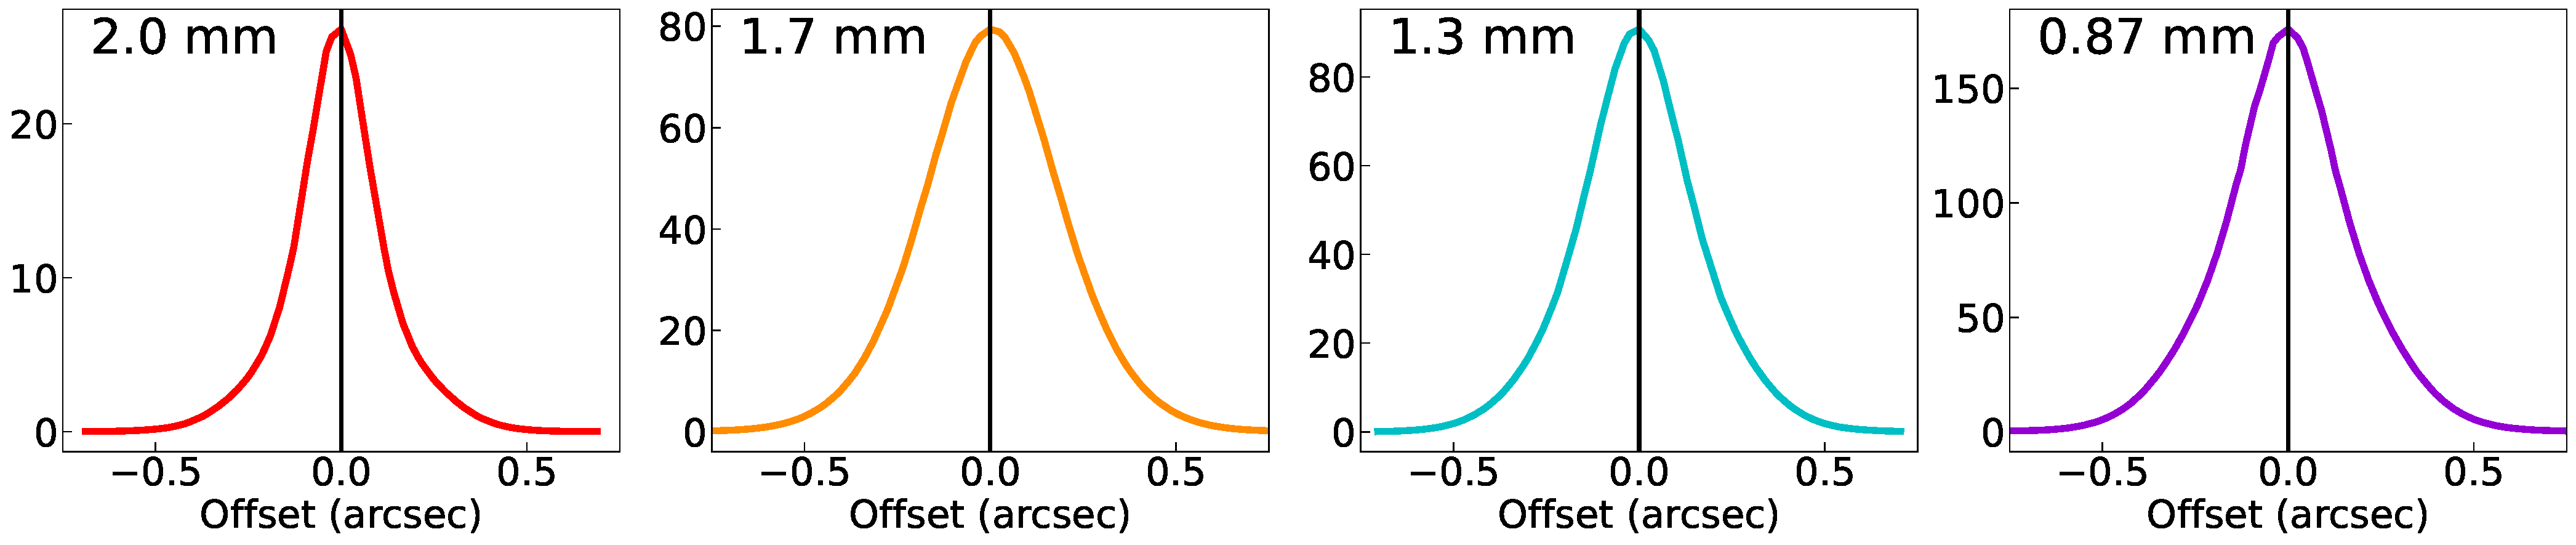
\includegraphics[width=1.1\textwidth]{WRITEUP_AND_IMAGES/IMAGES/WRITEUP/Slices/MW_slices_StokesI.pdf}
  \caption{Plot of Stokes I in mJy versus offset from the centre position of the disk. The centre position values can be found in Figure \ref{tab: source_info}, and the slices are shown in Figure \ref{fig: slice-along-minor}. A solid black line is shown at a offset of 0. }
  \label{fig: slices_StokesI}
\end{figure*}


\begin{figure*}[h]
  \centering
  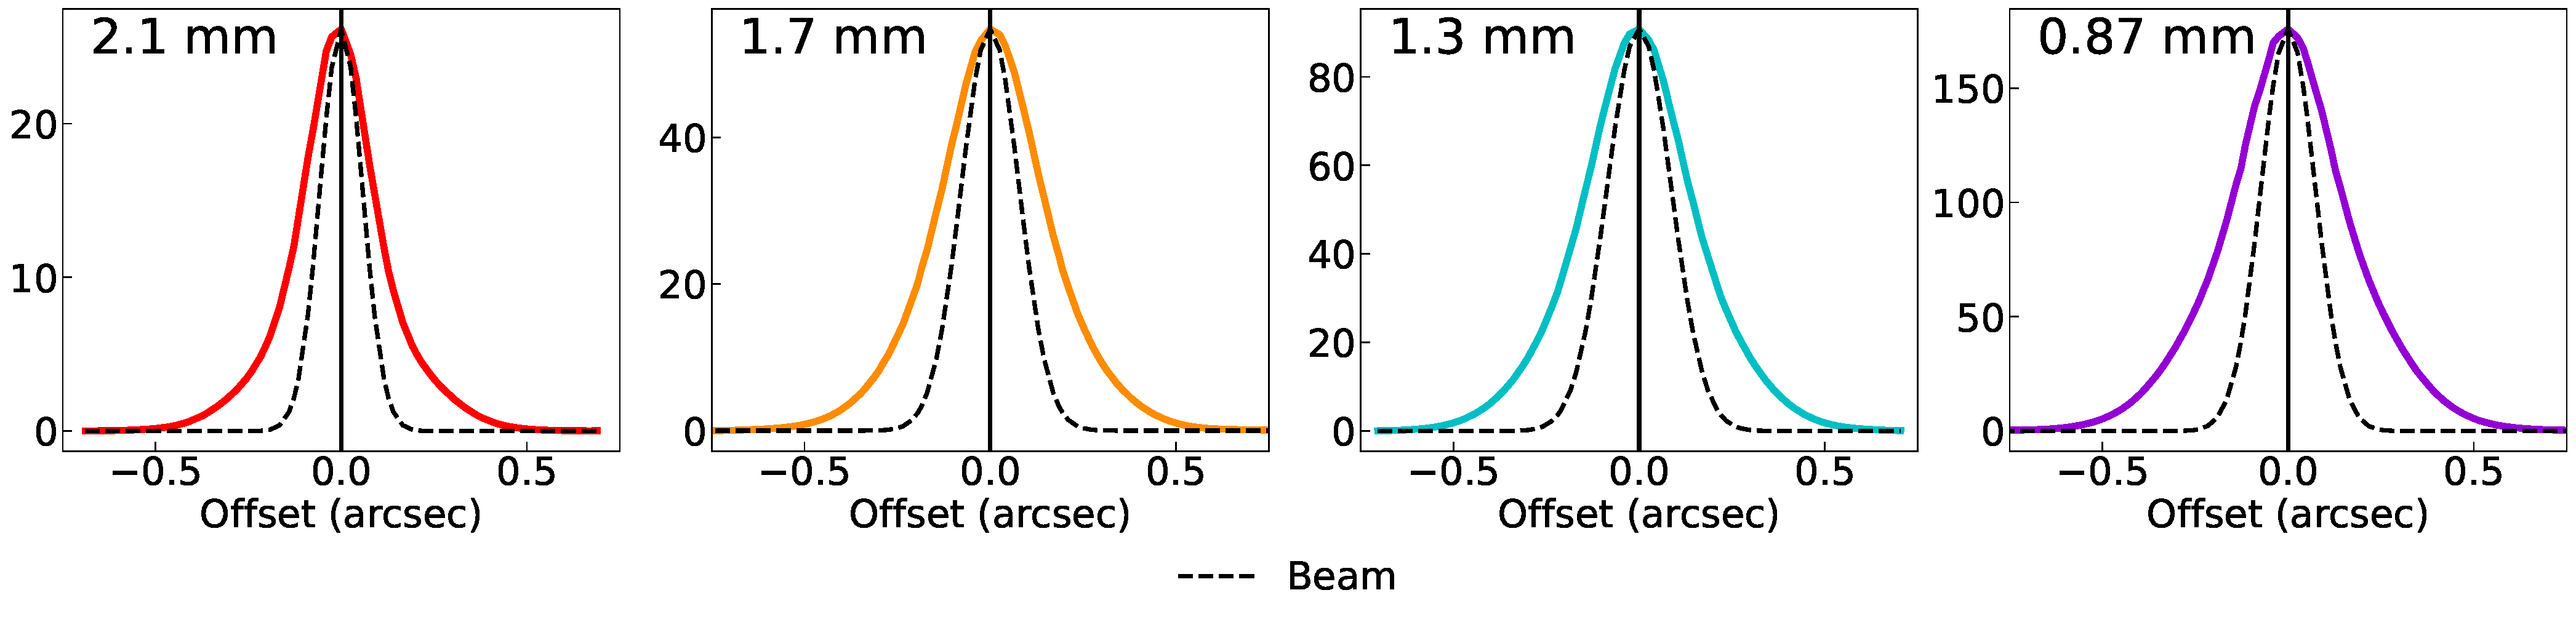
\includegraphics[width=1.1\textwidth]{WRITEUP_AND_IMAGES/IMAGES/WRITEUP/Slices/MW_slices_StokesI_with_beam.pdf}
  \caption{\question{Show plot with or without beam?}}
\end{figure*}

% ------------------------------------------------
\subsection{POLI}
% ------------------------------------------------
In Figure \ref{fig: slices_POLI} we present plots of the \POLI values along the slices along the minor axis for all 4 bands. When we look at the slices of \POLIns, we see some features that are different than \SIns. Primarily that the curves are no longer centred at (0,0), and that they all have a slight shift to the right. 
\begin{figure*}[h]
  \centering
  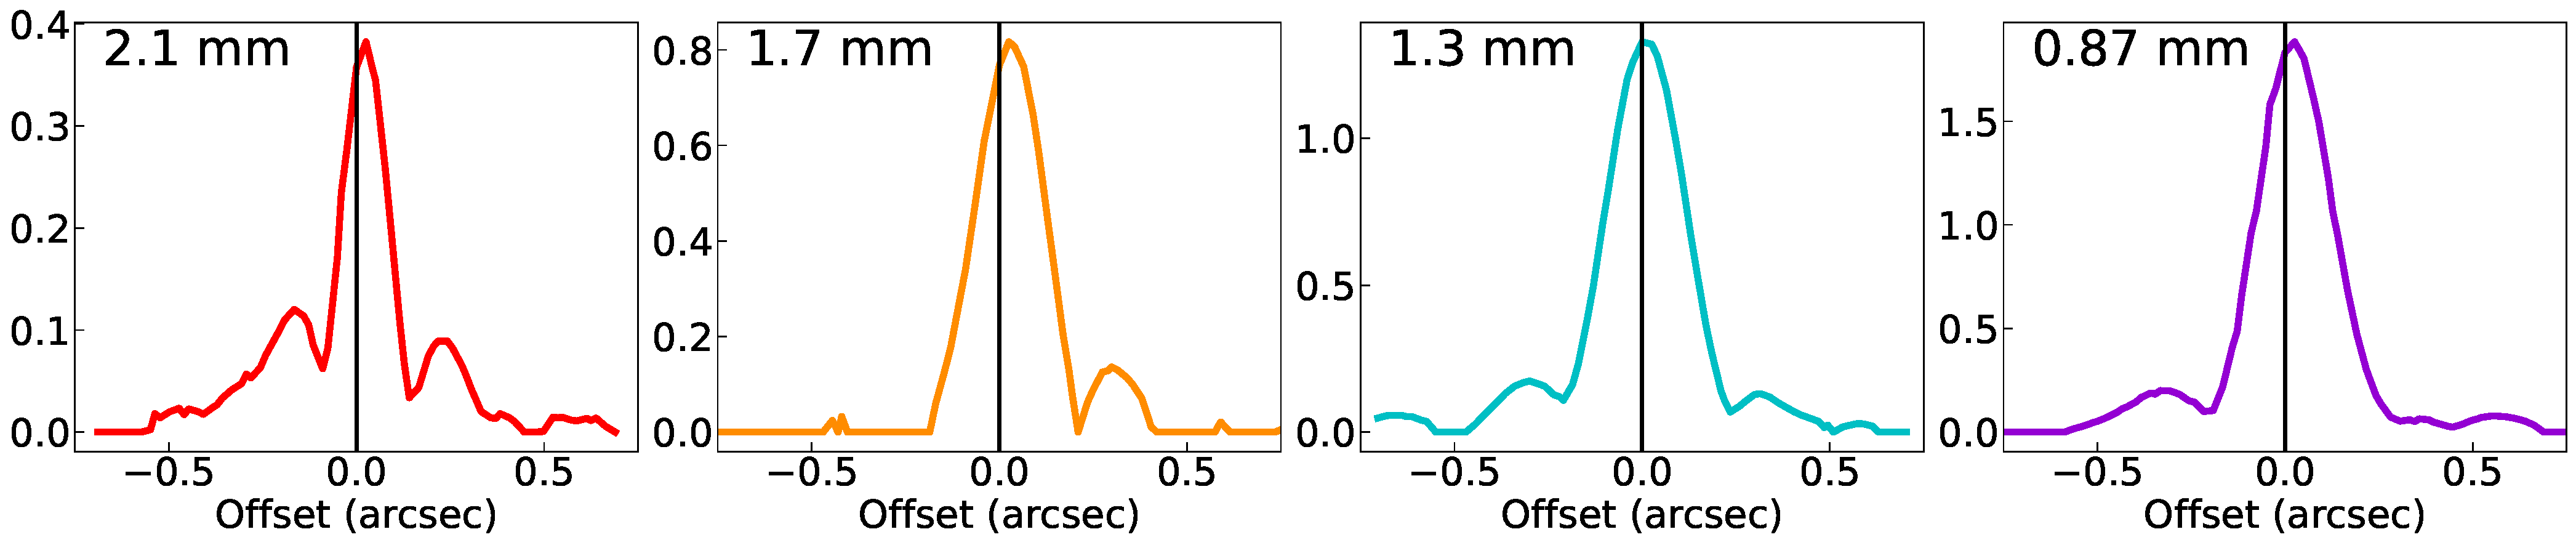
\includegraphics[width=1.1\textwidth]{WRITEUP_AND_IMAGES/IMAGES/WRITEUP/Slices/MW_slices_POLI.pdf}
  \caption{Same as Figure \ref{fig: slices_StokesI}, but for POLI.}
  \label{fig: slices_POLI}
\end{figure*}


\begin{figure*}[h]
  \centering
  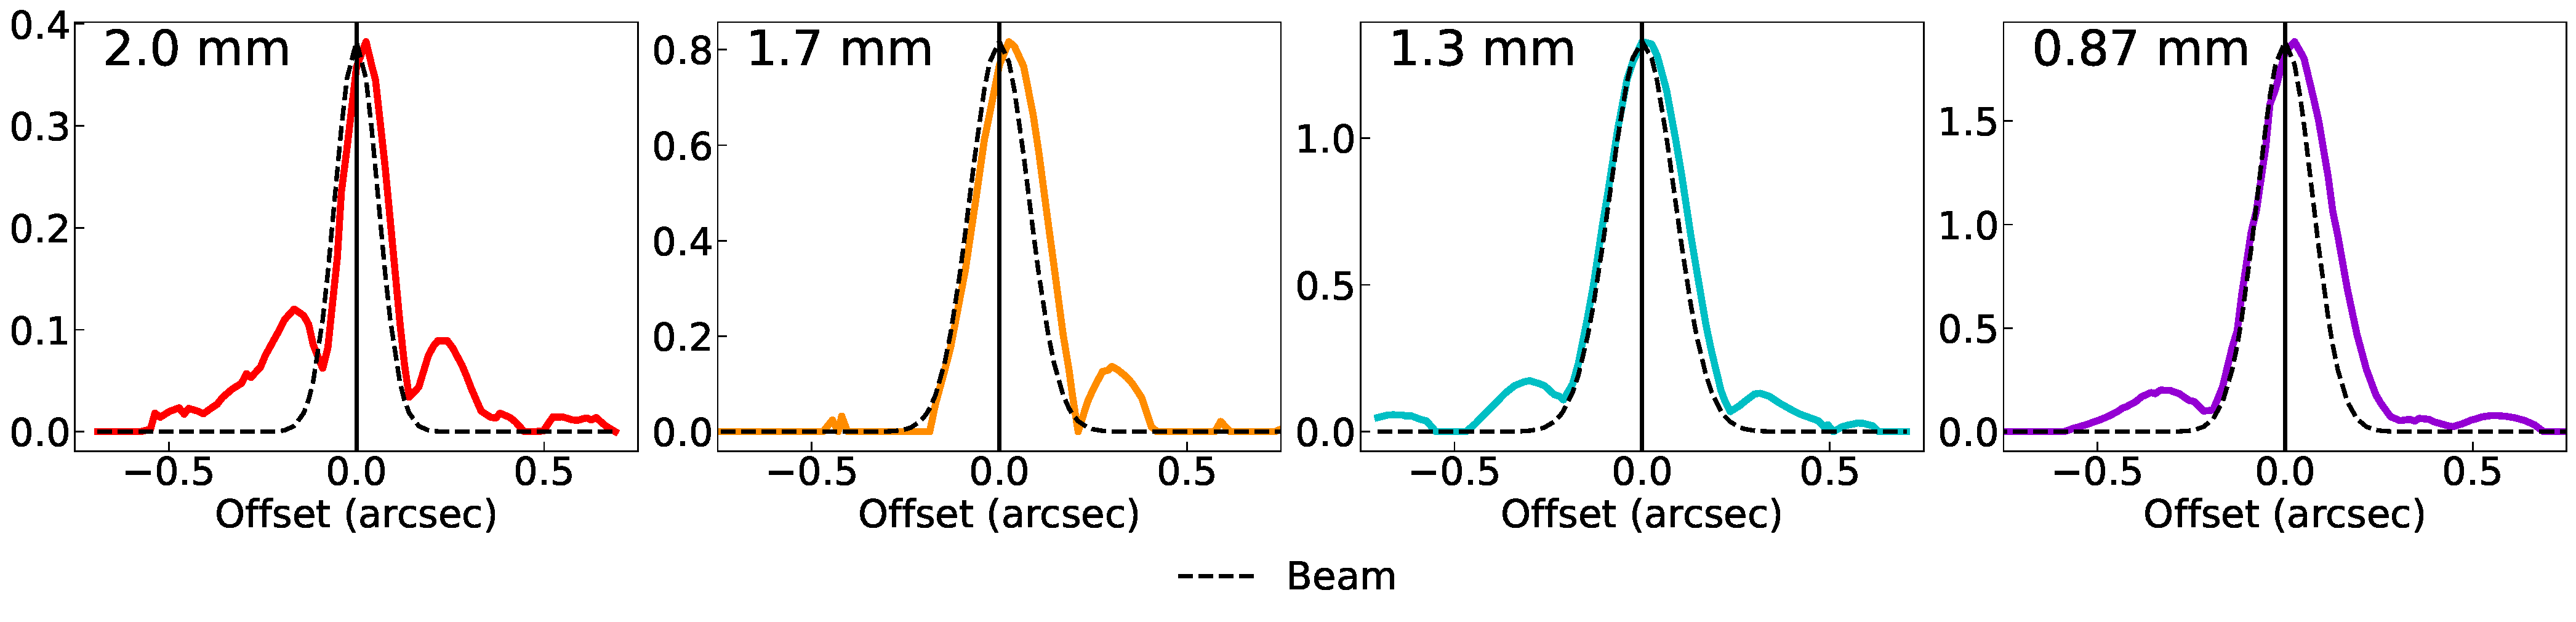
\includegraphics[width=1.1\textwidth]{WRITEUP_AND_IMAGES/IMAGES/WRITEUP/Slices/MW_slices_POLI_with_beam.pdf}
  \caption{\question{Show plot with or without beam?}}
\end{figure*}
% ------------------------------------------------
% ------------------------------------------------
% \section{POLF}
% ------------------------------------------------
% \begin{figure*}[h]
%   \centering
%   \includegraphics[width=1.1\textwidth]{WRITEUP_AND_IMAGES/IMAGES/WRITEUP/IRS63_mw_slice_POLF_writeup.jpeg}
%   \caption{\textcolor{red}{Add caption.}}
%   \label{fig: }
% \end{figure*}
